\subsection{Visão Geral}
O Sistema possuirá duas interfaces, sendo elas a de administrador e a do cliente.
A  interface  do  administrador  é  usada  pelo  administrador  do  sistema  para  criar, editar, listar ou visualizar as publicações. Enquanto a interface de cliente apresenta ao  usuário  uma  tela  com  as  informações  criadas,  comentários  feitos  nas  redes  sociais e um link em formato QR para que acessar a página \textit{web} da publicação.


\subsection{Interface de usuário}
\begin{table}[H]
\caption{Interfaces de Usuário}
\begin{tabularx}{\textwidth}{|c|X|}
\hline
Nome & \multicolumn{1}{c|}{Descrição} \\ \hline
Interface de administrador (logar) & Tela inicial apresentada quando se quer acessar as funcionalidades de administrador. \\ \hline
Interface do administrador (Inserir) & Interface para criação das novas publicações que serão exibidas para o cliente. \\ \hline
Interface do administrador (Listar) & Interface que lista todas as publicações criadas até o momento na tela de criação. \\ \hline
Interface do administrador (Editar) & Interface que possibilita a edição de alguns dados que foram inseridos. \\ \hline
Interface do administrador (Detalhar) & Interface que apresenta os detalhes de cada publicação criada. \\ \hline
Interface do Cliente & Interface onde é possível o cliente visualizar e acessar a publicação criada. \\ \hline
\end{tabularx}
\end{table}

    \subsubsection{Interface do administrador (Logar)}
    \begin{itemize}
        \item Leiaute
            \begin{figure}[H]
                \centering
                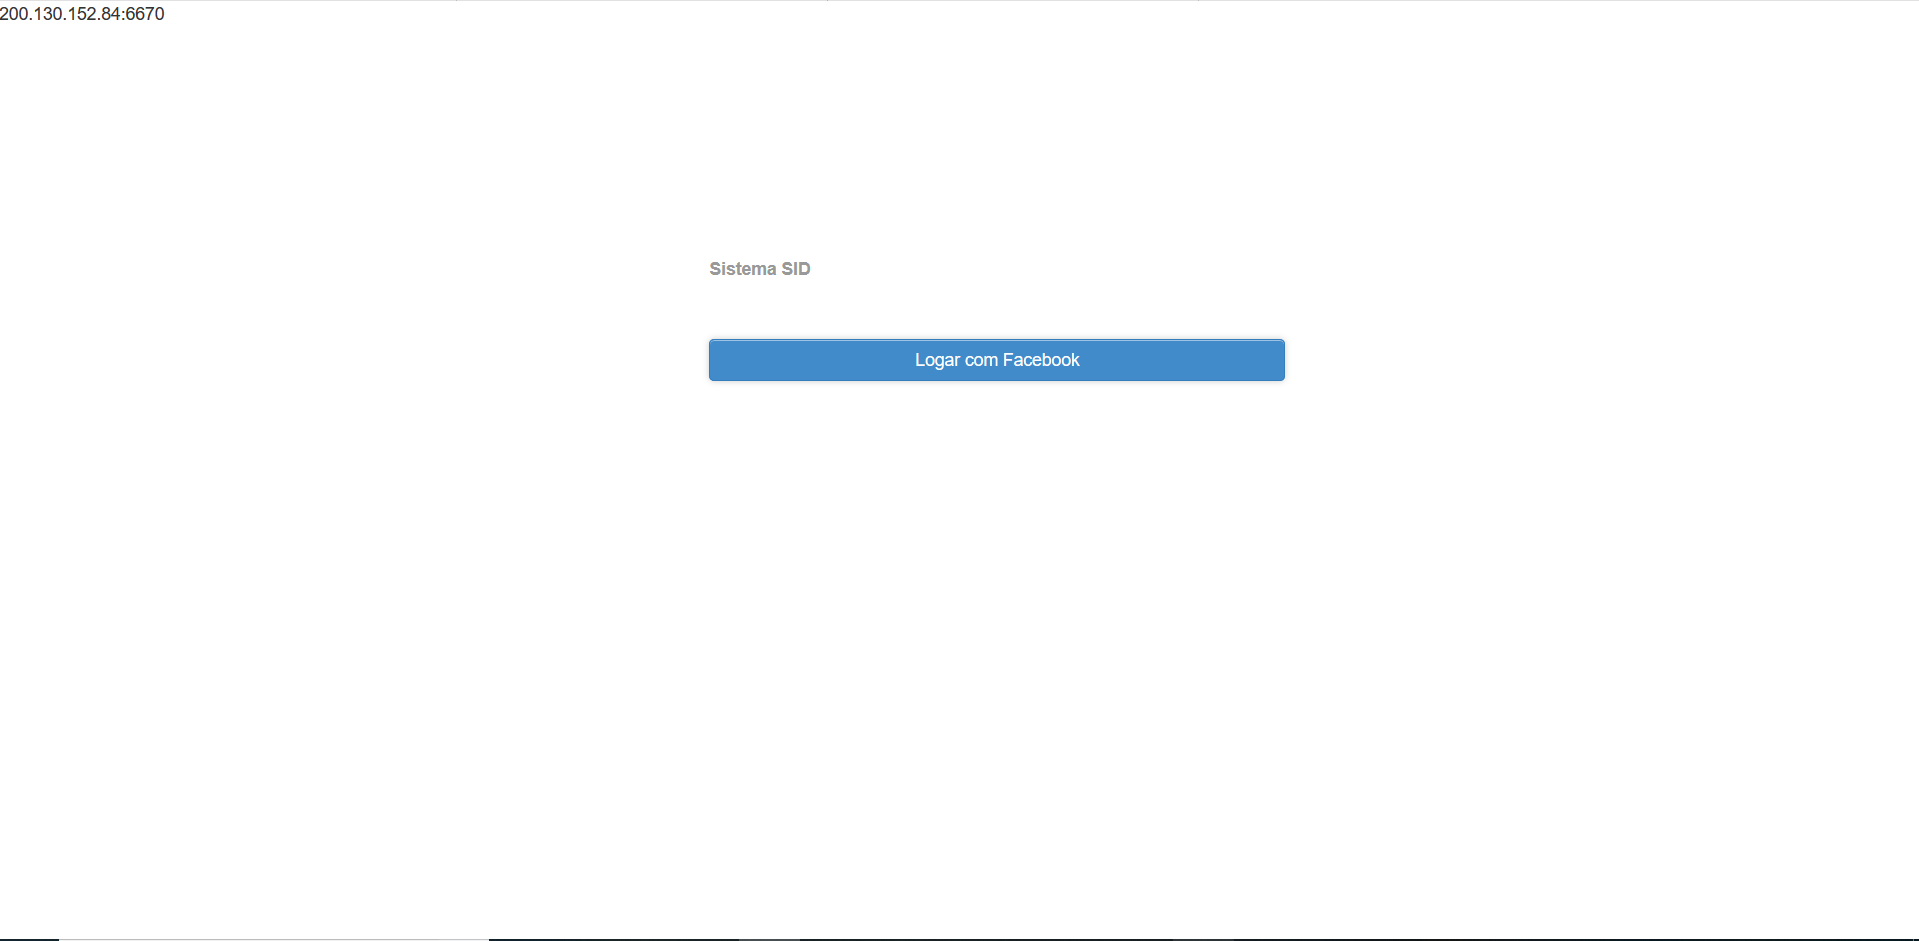
\includegraphics[width=\textwidth]{figuras/telalogar}
                \caption{Tela de login do Administrador}
            \end{figure}
        \item Campos\\
            Não se aplica.
        \item Comandos
            \begin{table}[H]
                \caption{Comandos da tela de logar}
                
                \begin{tabular}{|p{2cm}|p{3.3cm}|p{1.1cm}|p{3.9cm}|p{3.5cm}|}
                \hline
Nome & Descrição & Grupo & Requisitos de validade & Requisitos Diversos \\ \hline
Logar com Facebook & Usa a conta do Facebook do usuário para fazer login. & 
Todos & Autoriza se a conta estiver registrada 
no banco. & Deve possuir uma conta no Facebook. \\ \hline
                \end{tabular}
                
            \end{table}
    \end{itemize}
        
    \subsubsection{Interface do Administrador (Inserir)}
       \begin{itemize}
        \item Leiaute
            \begin{figure}[H]
                \centering
                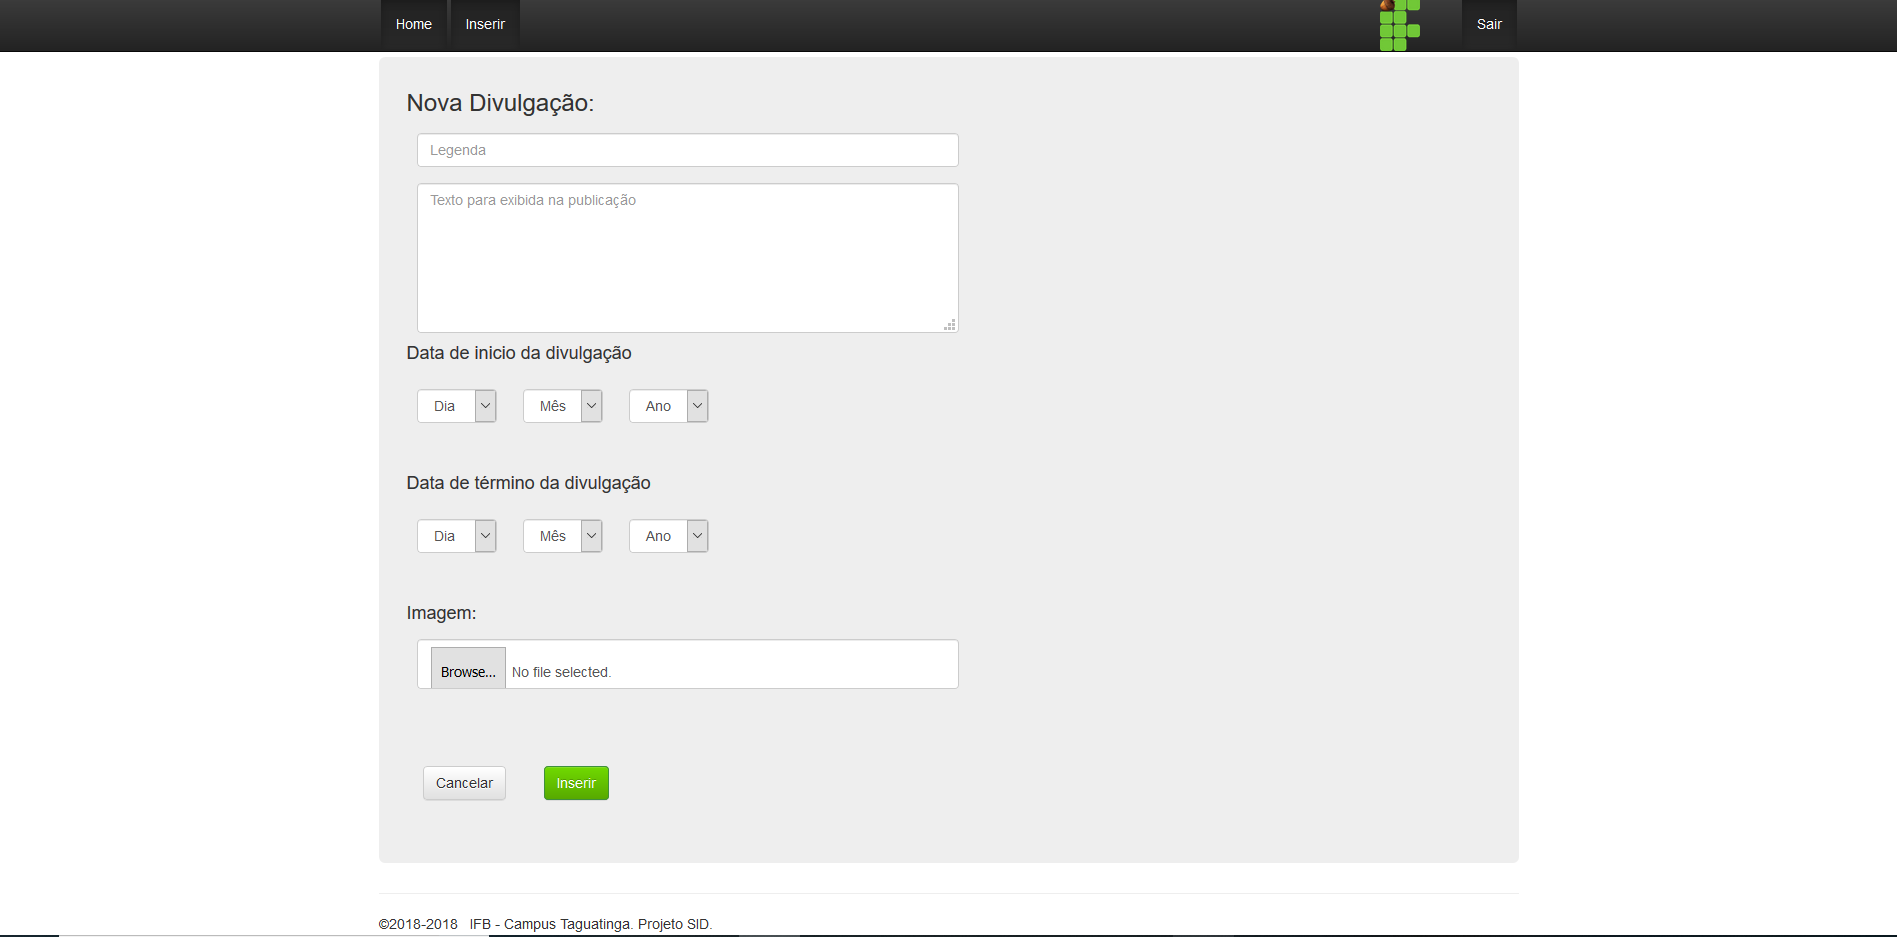
\includegraphics[width=\textwidth]{figuras/telainserir}
                \caption{Tela de inserção de novas publicações}
            \end{figure}
        
        \item Campos
        \begin{table}[H]
            \caption{Campos da tela de inserção}
                \begin{tabular}{|p{1.5cm}|p{3cm}|p{1.1cm}|p{3cm}|p{2.2cm}|p{2.5cm}|}
                \hline
Nome & Descrição & Grupo & Requisitos de conteúdo & Requisitos de edição & Requisitos Diversos \\ \hline
Legenda & Legenda que irá ser apresentada no cliente. & Admin & Texto & -- & -- \\ \hline
Texto & Texto da publicação que será postada no Facebook. & Admin & Texto & -- & -- \\ \hline
Data de início & Data em que a publicação começará a ser exibida no cliente. & Admin & Inteiro selecionável entre as opções apresentadas & -- & -- \\ \hline
Data de Término & Data em que a publicação deixará de ser exibida no cliente. & Admin & Inteiro selecionável entre as opções apresentadas & -- & -- \\ \hline
Imagem & Imagem que irá ser apresentada na publicação do Facebook e no Cliente. & Admin & Arquivo do tipo imagem. & -- & A imagem deve ter o formato suportado pelo Facebook \\ \hline
                \end{tabular}
            \end{table}
        \item Comandos
            \begin{table}[H]
                \caption{Comandos da tela de inserção}
                \begin{tabular}{|p{2cm}|p{4.7cm}|p{1.1cm}|p{3.9cm}|p{2cm}|}
                \hline
Nome & Descrição & Grupo & Requisitos de validade & Requisitos Diversos \\ \hline
Inserir & Insere no banco e no Facebook as informações descritas nos campos. & admin & Todos os campos devem estar preenchidos. &  \\ \hline
Cancelar & Cancela a inserção dos dados e retorna para a lista de publicações criadas. & admin &  &  \\ \hline
                \end{tabular}%
            \end{table}
    \end{itemize}
        
    \subsubsection{Interface do Administrador (Listar)}
        \begin{itemize}
        \item Leiaute
            \begin{figure}[H]
                \centering
                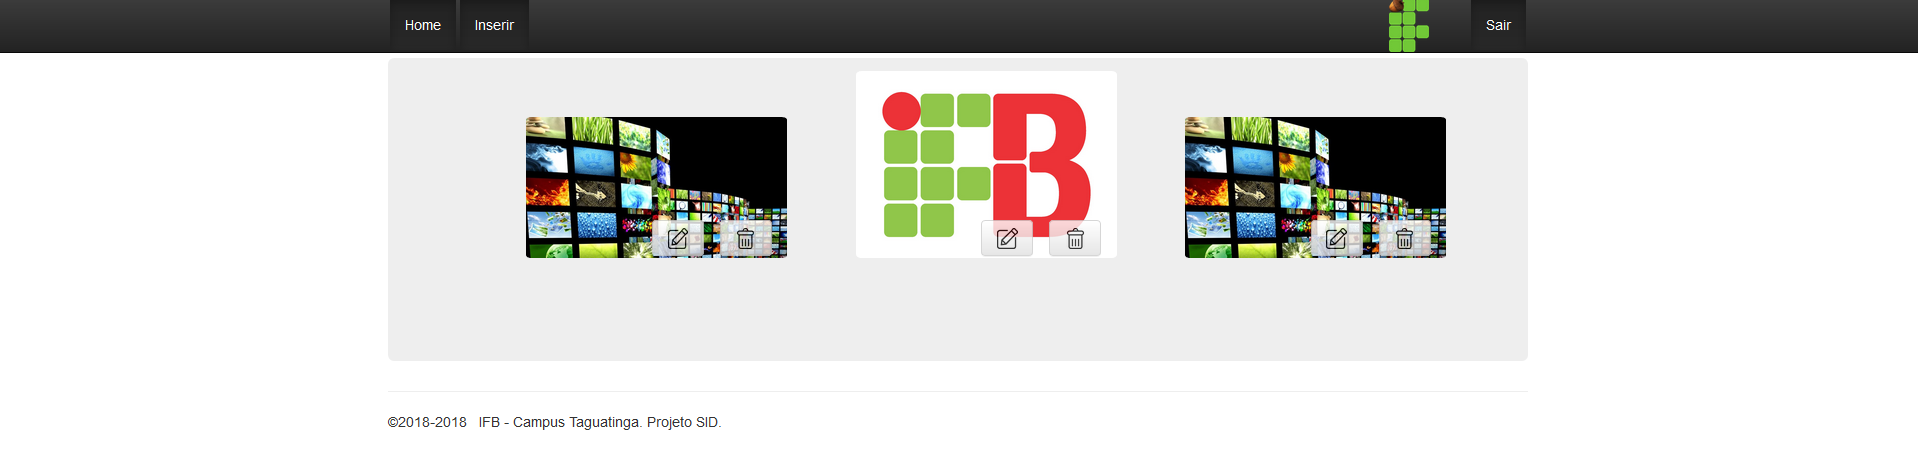
\includegraphics[width=\textwidth]{figuras/telalistar}
                \caption{Tela de listagem das publicações}
            \end{figure}
        \item Campos\\
            Não se aplica.
        \item Comandos
                \begin{table}[H]
                \caption{Comandos da tela de listagem}
                \resizebox{\textwidth}{!}{%
                \begin{tabular}{|p{2cm}|p{4.7cm}|p{1.1cm}|p{3.9cm}|p{2cm}|}
                \hline
Nome & Descrição & Grupo & Requisitos de validade & Requisitos Diversos \\ \hline
Detalhar & Clicar sobre a imagem retorna a páginacom  detalhes da publicação. & admin & -- & -- \\ \hline
Editar & O ícone de editar, retorna pagina de edição. & admin & -- & -- \\ \hline
Deletar & O ícone de excluir, exclui a publicação do banco e do Cliente. & admin & -- & -- \\ \hline
                \end{tabular}%
                }
            \end{table}
    \end{itemize}
        
    \subsubsection{Interface do Administrador (Editar)}
        \begin{itemize}
        \item Leiaute
            \begin{figure}[H]
                \centering
                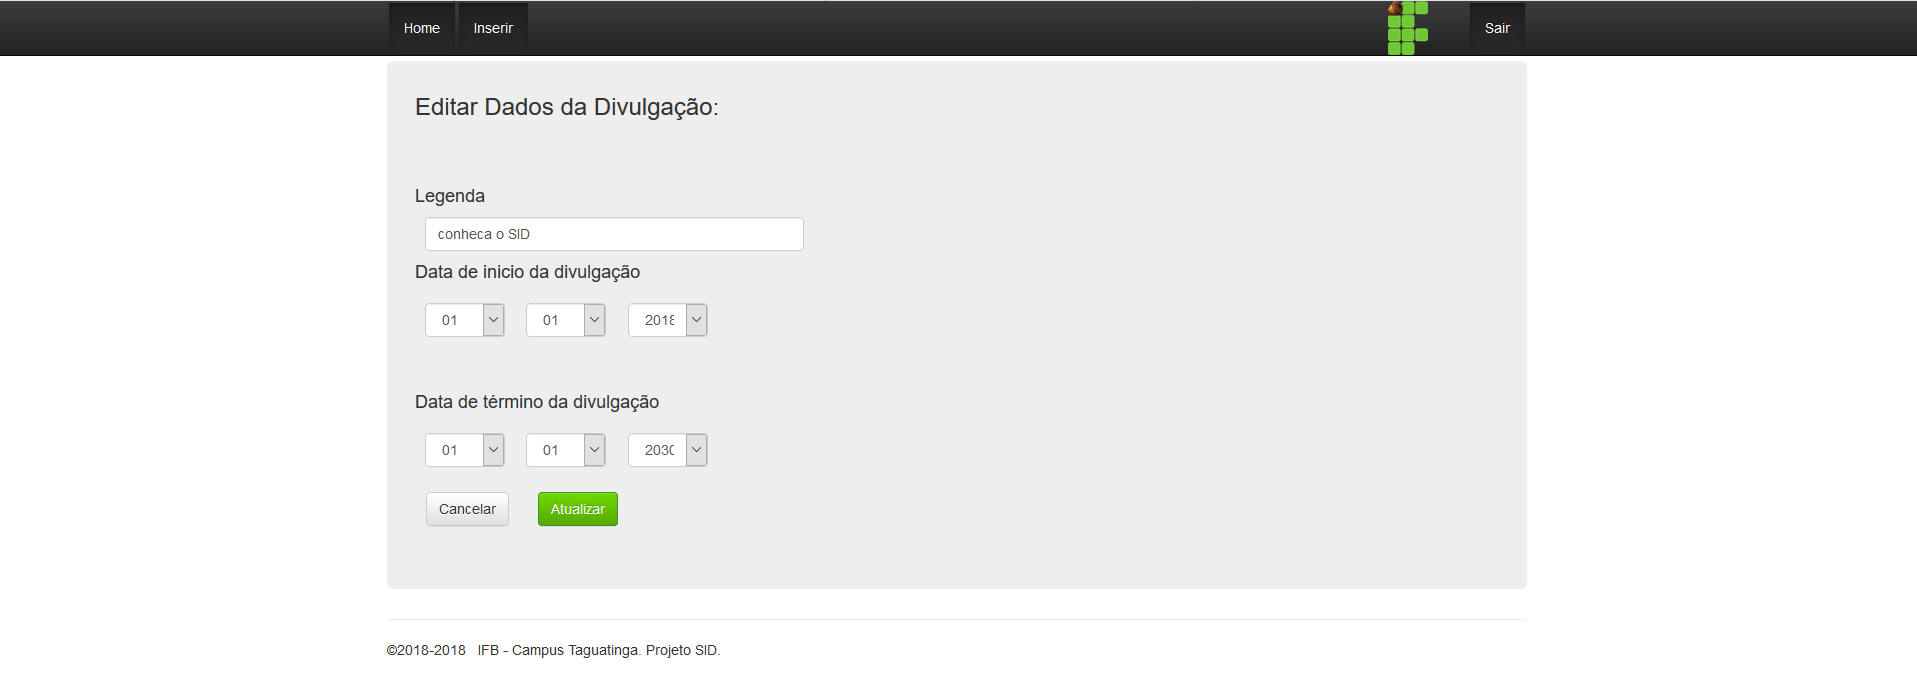
\includegraphics[width=\textwidth]{figuras/telaeditar}
                \caption{Tela de edição das publicações}
            \end{figure}
        \item Campos
\begin{table}[H]
            \caption{Campos da tela de edição}

                \begin{tabular}{|p{1.5cm}|p{3cm}|p{1.1cm}|p{3cm}|p{2.2cm}|p{2.5cm}|}
                \hline
Nome & Descrição & Grupo & Requisitos de conteúdo & Requisitos de edição & Requisitos Diversos \\ \hline
Legenda & Legenda que irá ser apresentada no cliente. & Admin & Texto & -- & -- \\ \hline
Data de início & Data em que a publicação começará a ser exibida no cliente. & Admin & Inteiro selecionável entre as opções apresentadas & -- & -- \\ \hline
Data de Término & Data em que a publicação deixará de ser exibida no cliente. & Admin & Inteiro selecionável entre as opções apresentadas & -- & -- \\ \hline
                \end{tabular}%
            \end{table}
        \item Comandos
            \begin{table}[H]
                \caption{Comandos da tela de edição}
                \begin{tabular}{|p{2cm}|p{4.7cm}|p{1.1cm}|p{3.9cm}|p{2cm}|}
                \hline
Nome & Descrição & Grupo & Requisitos de validade & Requisitos Diversos \\ \hline
Atualizar & Realiza a atualização no banco com os novos dados & admin & Todos os campos devem estar preenchidos & -- \\ \hline
Cancelar & Cancela as alterações e retorna a página de listagem & admin & -- & -- \\ \hline
                \end{tabular}%

            \end{table}
    \end{itemize}
        
    \subsubsection{Interface do Administrador (Detalhar)}
        \begin{itemize}
        \item Leiaute
            \begin{figure}[H]
                \centering
                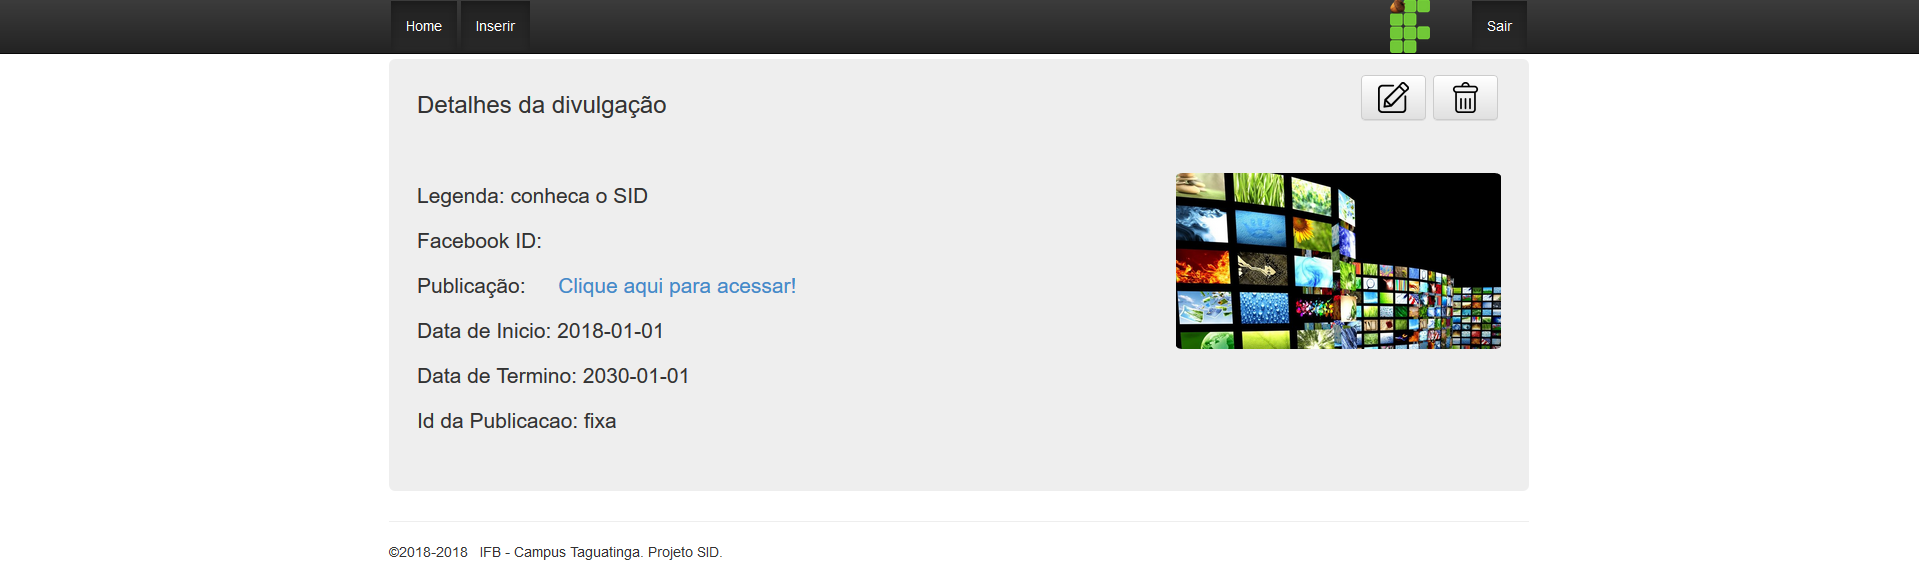
\includegraphics[width=\textwidth]{figuras/teladetalhar}
                \caption{Tela de detalhamento das publicações}
            \end{figure}
        \item Campos\\
            Não se aplica.
        \item Comandos
            \begin{table}[H]
                \caption{Comandos da tela de detalhamento}
                \resizebox{\textwidth}{!}{%
                \begin{tabular}{|p{2cm}|p{4.7cm}|p{1.1cm}|p{3.9cm}|p{2cm}|}
                \hline
Nome & Descrição & Grupo & Requisitos de validade & Requisitos Diversos \\ \hline
Clique Aqui & Acessa aolink da publicação no Facebook. & admin & -- & -- \\ \hline
Editar & O ícone de editar, retorna pagina de edição. & admin & -- & -- \\ \hline
Deletar & O ícone de excluir, exclui a publicação do banco e do Cliente. & admin & -- & -- \\ \hline
                \end{tabular}%
                }
            \end{table}
    \end{itemize}
        
    \subsubsection{Interface Cliente}
        \begin{itemize}
        \item Leiaute
            \begin{figure}[H]
                \centering
                
\includegraphics[width=\textwidth]{figuras/telacliente}
                \caption{Tela do cliente}
            \end{figure}
        \item Campos\\
            Não se aplica.
        \item Comandos\\
            Não se aplica.
        \end{itemize}